\documentclass[a4paper,12pt]{article}
\usepackage[utf8]{inputenc}
\usepackage{amsmath}
\usepackage{amsfonts}
\usepackage{amssymb}
\usepackage{graphicx}
\usepackage{caption}
\usepackage{subcaption}
\usepackage{float}
\usepackage{siunitx}
\usepackage{booktabs}
\usepackage{hyperref}

\title{Esperimento Michelson}
\author{Francesco Giuseppe Minisini, Mattia Monzani, Gabriele Turi}
\date{January 13, 2025}

\begin{document}

\maketitle
\hrule
\vspace{9pt}
\begin{abstract}
    \noindent
    Nell'esperimento condotto sono state effettuate misure ottiche di precisione tramite un interferometro di Michelson. Si è misurata la lunghezza d’onda di un laser rosso \((632 \pm 14)\,\text{nm}\), corretta per l’indice di rifrazione dell’aria \((634 \pm 15)\,\text{nm}\). Si è determinato l’indice di rifrazione dell’aria \((1.000275 \pm 0.000006)\). Successivamente abbiamo ottenuto la lunghezza di coerenza della luce bianca \((6.2 \pm 0.9)\,\mu\text{m}\). Inoltre, si è ricavato lo scarto fra le due lunghezze d’onda del doppietto del sodio \((6.033 \pm 0.018)\,\text{\AA}\), ottenendo risultati in buon accordo con i dati noti.
\vspace{20 pt}
\hrule
\end{abstract}
\vspace{2 pt}


\section{Messa a punto dell'apparato sperimentale}
L’interferometro di Michelson, rappresentato nello schema di Figura \ref{fig:apparato_completo}, è costituito dalla lastra semiriflettente \(S_1\), dagli specchi completamente riflettenti \(S_2\) e \(S_3\), e dalla lastra di compensazione Lc. Le superfici ottiche sono lavorate con precisione per garantire planarità e ridurre asperità a dimensioni comparabili alla lunghezza d’onda della luce visibile. Gli specchi \(S_2\) e \(S_3\) sono montati su supporti regolabili con viti micrometriche per consentire l’ortogonalità reciproca, fondamentale per ottenere figure di interferenza accurate.

\begin{figure}[H]
    \centering
    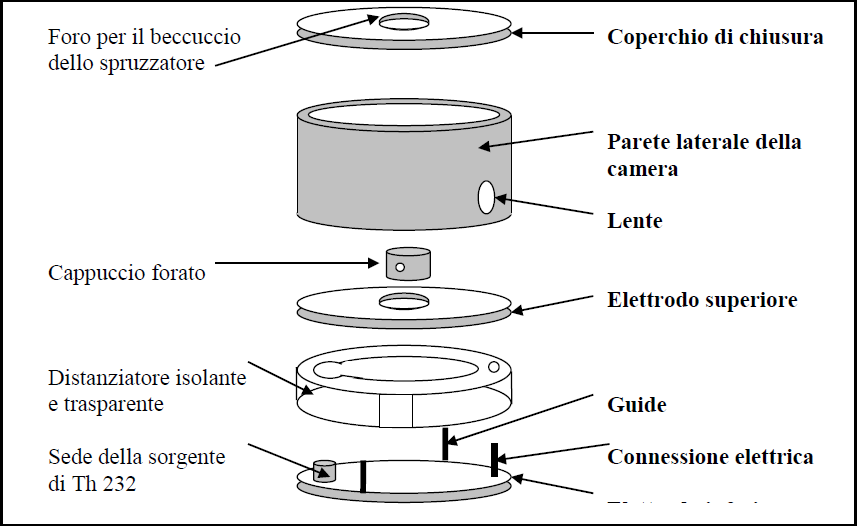
\includegraphics[width=0.6\textwidth]{Apparato2.png}
    \caption{Schema dell'apparato sperimentale completo.}
    \label{fig:apparato_completo}
\end{figure}

Lo specchio \(S_3\), inoltre, è montato su un carrello mobile che consente spostamenti controllati con sensibilità fino a 2000 nm. La sorgente luminosa, montata su un banco ottico separato, come illustrato nella Figura \ref{fig:Sistema_lenti}, ed è orientata in modo da garantire l’incidenza a 45° sulla lastra semiriflettente \(S_1\). Il fascio luminoso, suddiviso da \(S_1\) in due raggi distinti, percorre cammini separati riflettendosi sugli specchi \(S_2\) e \(S_3\). I due raggi si sovrappongono successivamente sullo schermo, formando una figura di interferenza dovuta alla coerenza ottica dei raggi generati da una sorgente comune.

\begin{figure}[H]
    \centering
    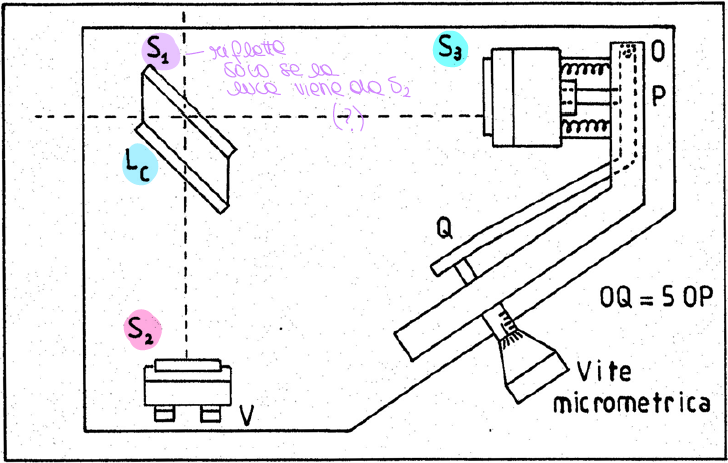
\includegraphics[width=0.7\textwidth]{apparato1.png}
    \caption{Sistema di lenti dell'apparato sperimentale.}
    \label{fig:Sistema_lenti}
\end{figure}

Prima dell’acquisizione dei dati, è necessario calibrare l’apparato regolando l’ortogonalità tra gli specchi \(S_2\) e \(S_3\). La procedura prevede di sovrapporre sullo schermo le immagini riflesse dagli specchi tramite le viti micrometriche di \(S_2\), eliminando riflessioni parassite mediante ostacoli interposti nei percorsi ottici \(S_1\)-\(S_2\) e \(S_1\)-\(S_3\). Una volta completata questa fase, si utilizza una lente divergente per espandere il fascio luminoso e rendere le figure di interferenza più facilmente osservabili. 

E' possibile notare che posizionare la lente troppo vicina alla sorgente ne aumenta la dimensione ma ne diminuisce l’intensità, mentre posizionarla troppo vicina allo specchio \(S_1\) non ne varia la dimensione. Si sceglie quindi una posizione in cui la larghezza del fascio è massima e tutta la luce incide sullo specchio \(S_1\). Regolando con precisione le viti di \(S_2\), si ottengono frange circolari, segno della corretta ortogonalità degli specchi. La circolarità delle frange è il risultato dell’intersezione sullo schermo di iperboloidi di rotazione generati dalle sorgenti virtuali F3 e F2', immagini degli specchi \(S_3\) e \(S_2\) rispettivamente. 

Al diminuire della differenza dei cammini ottici, il numero delle frange si riduce e il loro spessore aumenta, fino a scomparire nella condizione di cammini ottici equivalenti. Se gli specchi non sono perfettamente ortogonali, le frange circolari si trasformano in ellissi o porzioni di ellissi, con una geometria che varia a seconda dell'inclinazione degli specchi e della distanza tra i fuochi degli iperboloidi. 

In queste condizioni, traslando lo specchio \(S_3\), si può individuare la condizione di equidistanza degli specchi, caratterizzata dal passaggio da frange ellittiche a frange rettilinee. Ulteriori spostamenti dello specchio oltre questa condizione portano a una variazione del verso della concavità delle frange, un aspetto che può essere sfruttato per identificare con precisione la zona di equidistanza. Questa calibrazione consente di eseguire misurazioni precise delle variazioni di cammino ottico, che si riflettono in cambiamenti osservabili nella geometria delle figure di interferenza.


\section{Misurazione della lunghezza d’onda del laser}
Una prima misurazione che è possibile effettuare con un interferometro di Michelson è quella della determinazione della lunghezza d’onda di un laser osservando il comportamento del pattern di interferenza che la luce del laser produce su uno schermo in seguito all’attraversamento dell’apparato. Si può configurare correttamente l’apparato in modo che si visualizzino fronti d’onda dall’aspetto circolare e si può prendere in considerazione la relazione che si ottiene imponendo che la differenza di cammino ottico tra i due raggi derivanti dallo sdoppiamento del raggio iniziale sia uguale ad un multiplo intero della lunghezza d’onda della luce utilizzata, in modo da visualizzare in un dato punto dello schermo un’interferenza costruttiva: 
\begin{equation}
2d n \cos\theta = m\lambda,
\label{eq:interferenza_costruttiva}
\end{equation}
dove:
\begin{itemize}
    \item \( d \) è la distanza tra \(S_3\) e l'immagine virtuale di \(S_2\) prodotta da \(S_1\)
    \item \( n \) è l’indice di rifrazione del mezzo di propagazione della luce
    \item \( \theta \) è la posizione angolare, rispetto alla normale, al centro del pattern dello schermo, di un certo punto in cui vi è interferenza costruttiva
    \item \( m \) è un numero intero
    \item \( \lambda \) è la lunghezza d’onda della luce impiegata
\end{itemize}
Variando \( d \), mediante la vita micrometrica su \( S_3\), varia la differenza di cammino ottico e di conseguenza cambia la posizione dei punti in cui si ha interferenza costruttiva. Questo porta a uno scorrimento delle frange sullo schermo.

Si noti che la differenza di cammino ottico in corrispondenza di una certa posizione angolare sullo schermo è data da:
\begin{equation}
2d n \cos\theta.
\end{equation}
Se lo specchio subisce uno spostamento \( \Delta x \), allora la variazione della differenza di cammino ottico è:
\begin{equation}
2\Delta x n \cos\theta.
\label{eq:variazione_cammino}
\end{equation}
Per un opportuno valore di \( \Delta x \), la differenza di cammino ottico può variare di un valore pari a \( \lambda \), il che consente di visualizzare nuovamente massimi di interferenza negli stessi punti, poiché la differenza di cammino ottico diventa un multiplo intero di \( \lambda \).
Se si osservano \( N \) frange attraversare il centro del pattern (\( \theta = 0 \implies \cos\theta = 1 \)) a seguito di una variazione \( \Delta x \) della posizione dello specchio, si ha la relazione:

\begin{equation}
2\Delta x n = N\lambda,
\label{eq:frange_interferenza}
\end{equation}
da cui si ricava:
\begin{equation}
\lambda = \frac{2\Delta x n}{N}.
\label{eq:calcolo_lambda}
\end{equation}

I valori di \( \lambda \) sono stati mediati per ottenere una stima migliore. Nelle misurazioni si è temporaneamente considerato l’indice di rifrazione dell’aria pari a 1.
La variazione \( \Delta x \) è calcolata come:
\begin{equation}
\Delta x = |x_f - x_i|,
\end{equation}
dove \( x_f \) e \( x_i \) sono rispettivamente le posizioni finale e iniziale dello specchio. L’incertezza su \( \Delta x \) è esprimibile, per propagazione degli errori, come:

\begin{equation}
\sigma_{\Delta x} = \sqrt{\sigma_{x_i}^2 + \sigma_{x_f}^2},
\label{eq:incertezza_delta_x}
\end{equation}
dove l’incertezza sulle posizioni dello specchio è stata considerata pari alla sensibilità del nonio montato sul carrello mobile che è stato usato per misurare le posizioni di S3 (\( 2 \, \mu\text{m} \)). Per il numero di frange \( N \) è stata considerata un’incertezza di 2 frange, dovuta a errori di conteggio umano. L’incertezza sulla lunghezza d’onda \( \lambda \) è stata calcolata tramite propagazione dell’errore:
\begin{equation}
    \sigma_{\lambda} = \sqrt{\left(\frac{\partial \lambda}{\partial N} \sigma_N\right)^2 + \left(\frac{\partial \lambda}{\partial \Delta x} \sigma_{\Delta x}\right)^2}
    \label{eq:incertezza_lambda}
\end{equation}

Per misurare \( \lambda \), sono state effettuate 8 misurazioni della posizione iniziale e finale dello specchio, osservando indicativamente 150 fasci di interferenza. 
Ottenendo infine la miglior stima con la media pesata:

\begin{equation}
\lambda = (632 \pm 14) \, \text{nm}.
\label{eq:valore_lambda}
\end{equation}
Questa misurazione rientra nel range noto della lunghezza d’onda della luce rossa, compreso tra \( [625, 750] \, \text{nm} \).

Avendo invece una stima dell’indice sull’indice di rifrazione dell’aria, è di conseguenza possibile calcolare la lunghezza d’onda del raggio laser utilizzando il valore dell’indice di rifrazione calcolato, senza approssimarlo ad 1. 
Nel seguente punto dell’esperimento, si è stimato l’indice di rifrazione dell’aria, e si è svolto nuovamente il calcolo (adattando la relazione \ref{eq:incertezza_lambda} aggiungendo il termine per la propagazione dell'errore di \(n\)), per determinare la lunghezza d’onda del laser, ottenendo come risultato: 

\begin{equation}
    \lambda = (634 \pm 15) \, \text{nm}.
    \label{eq:valore_lambda_2}
    \end{equation}

\section{Misurazione dell’indice di rifrazione dell’aria}

Un’altra misurazione che è possibile effettuare con l’interferometro di Michelson, una volta noto il valore della lunghezza d’onda del laser utilizzato, è quella dell’indice di rifrazione dell’aria.
Per condurre questa misura, si può iniziare anteponendo una camera cilindrica di lunghezza nota:
\[
D = (5.0 \pm 0.2) \, \text{cm},
\]
tra lo specchio parallelo allo schermo di visualizzazione della figura di interferenza e lo stesso schermo. Una pompa a vuoto viene utilizzata per aspirare l’aria presente nella camera, generando, entro una certa approssimazione, il vuoto (indice di rifrazione \(n_0 = 1\)) all’interno della camera, raggiungendo pressioni inferiori a \(10^{-1} \, \text{torr}\). In queste condizioni, sullo schermo si osserva una figura di interferenza con frange circolari.

Ruotando progressivamente una valvola, si può reintrodurre l’aria nella camera, variando così l’indice di rifrazione del volume interno. Questa variazione provoca un cambiamento nella differenza di cammino ottico dei due raggi, poiché essa dipende dall’indice di rifrazione delle regioni attraversate dai raggi luminosi. Di conseguenza, si osserva lo scorrimento delle frange di interferenza sullo schermo. Ogni volta che la differenza di cammino ottico varia di \( \lambda \), si nota il passaggio di una frangia per un punto.

Quando l’aria è stata completamente reintrodotta nella camera, il numero totale di interferenze costruttive osservate al centro del pattern (\(N\)) soddisfa la relazione:
\begin{equation}
\Delta L = N\lambda,
\label{eq:delta_cammino_ottico}
\end{equation}
dove \( \Delta L \) rappresenta la variazione complessiva della differenza di cammino ottico tra la condizione di vuoto e quella di camera piena. In particolare
\[
\Delta L = 2D (n_a - n_0),
\]
dove:
\begin{itemize}
    \item \( D \) la lunghezza della camera
    \item \( n_0 = 1 \) l'indice di rifrazione del vuoto
    \item \( n_a \) l'indice di rifrazione dell’aria
\end{itemize}
Dunque, invertendo la relazione, si ottiene l’indice di rifrazione dell’aria:

\begin{equation}
n_a = \frac{N\lambda}{2D} + 1,
\label{eq:indice_rifrazione}
\end{equation}
dove \( \lambda \) è la lunghezza d’onda del laser ottenuta nella misurazione precedente.
L’incertezza sul valore di \( n_a \) è determinata tramite propagazione degli errori:

\begin{equation}
\sigma_{n_a} = \sqrt{\left(\frac{\partial n_a}{\partial N} \sigma_N\right)^2 + \left(\frac{\partial n_a}{\partial \lambda} \sigma_\lambda\right)^2 + \left(\frac{\partial n_a}{\partial D} \sigma_D\right)^2},
\label{eq:incertezza_indice}
\end{equation}
dove:
\begin{itemize}
    \item \( \sigma_N \) è l’incertezza sul numero di frange, considerata pari a 2 frange per errore di conteggio
    \item \( \sigma_\lambda \) è l’incertezza sulla lunghezza d’onda (\( \pm 14 \, \text{nm} \))
    \item \( \sigma_D \) è l’incertezza sulla lunghezza della camera (\( \pm 0.2 \, \text{cm} \))
\end{itemize}
Sono stati effettuati 9 conteggi del numero di frange, e la media pesata dei valori ottenuti ha fornito la miglior stima dell’indice di rifrazione dell’aria:
\begin{equation}
n_a = 1.000275 \pm 0.000006.
\label{eq:valore_na}
\end{equation}
Ottenendo una compatibilità del \( 0.2 \, \% \), con il valore noto dell’indice di rifrazione dell’aria a condizioni di temperatura e pressione dell’aria standard (\( 1 \, \text{atm} \) di pressione dell’aria e temperatura ambiente), di \( 1.000293 \). La compatibilità ottenuta è ritenibile, in quanto al di sotto della soglia convenzionale di\(5\%\), non soddisfacente. 


È bene considerare che l'indice di rifrazione da noi misurato possa essere differente da quello noto: le condizioni di temperatura e pressione in corrispondenza di cui si attribuisce valore noto riportato dell'indice di rifrazione, possono non corrispondere a quelle presenti in laboratorio al momento dell'esperimento.
Indipendentemente da questa considerazione, si ipotizza che tale distanza dal valore di riferimento sia probabilmente imputabile alla sottostima dell’indice di rifrazione della camera nella condizione di aria risucchiata, con conseguente sottostima della misura dell’indice di rifrazione dell’aria. 

Difatti, per il calcolo effettuato per determinare l’indice di rifrazione dell’aria, si assume che l’indice di rifrazione all’interno della camera nelle condizioni di vuoto create sia esattamente \( 1 \), il che è un’approssimazione, in quanto all’interno della camera non vi è possibile riprodurre il vuoto perfetto (difatti, si stima vi rimanga un residuo d’aria a \( 10^{-1} \, \text{torr} \) di pressione). Dunque, la misura sull’indice di rifrazione risulta viziata dalla presenza di un errore sistematico non trascurabile sulla stima dell’indice di rifrazione del volume interno alla camera in condizioni di aria aspirata.

\section{Misurazione della lunghezza del pacchetto d’onda di luce bianca}
Se, anziché studiare il comportamento nell’interferometro di Michelson di un’onda luminosa coerente, si utilizza quello ad esempio della luce bianca emessa da una lampada ad incandescenza, allora si sta in questo caso studiando il caso di un’onda luminosa non coerente, ovvero un caso in cui la radiazione luminosa lungo la sua direzione di propagazione si concentra in modo discreto in lunghezze di pochi micrometri a formare il cosiddetto “pacchetto d’onda”. 

Dunque, una volta che un pacchetto di luce bianca attraversa lo specchio semi-riflettente sdoppiandosi in due semi-pacchetti, questi daranno vita ad una figura di interferenza sullo schermo solo se la differenza di lunghezza dei bracci dei due specchi riflettenti è minore della lunghezza di coerenza dei pacchetti di luce bianca. 
Quindi si procede innanzitutto a ruotare lo specchio ruotabile in modo da rompere la condizione di ortogonalità dei due specchi cercando di ottenere figure di interferenza il più possibili piane. In seguito, dopo che si è accesa la lampada ad incandescenza che emette luce bianca, si sposta lo specchio dotato del carrello micrometrico fino a quando non si osserva sullo schermo illuminato (su cui, in generale, senza avere interferenza dei due semi-pacchetti, si nota una normale illuminazione di colore bianco) la figura data dall’interferenza dei due semi-pacchetti d’onda (costituita da frange rettilinee colorate secondo lo spettro della radiazione-elettromagnetica visibile). 

Una volta raggiunta la condizione desiderata per cui è visibile l’interferenza dei semi-pacchetti d’onda, è possibile: 
Misurare la posizione limite dello specchio parallelo allo schermo in corrispondenza di cui si passa dalla visualizzazione della luce bianca alla visualizzazione della figura di interferenza. 
Variare in seguito la posizione dello specchio osservando lo scorrimento delle frange della figura di interferenza.
Misurare la posizione dello specchio in corrispondenza di cui si osserva il passaggio dalla visualizzazione della figura di interferenza alla visione nuovamente della luce bianca. 
Dunque, siccome i semi-pacchetti interferiscono se la differenza del loro cammino è minore della lunghezza del pacchetto e si cessa di visualizzare l’interferenza dei pacchetti d’onda non appena la differenza di cammino dei due pacchetti diventa maggiore della loro lunghezza si può stimare con buona approssimazione la lunghezza del pacchetto d’onda con lo spostamento applicato allo specchio da quando l’interferenza inizia ad essere visibile a quando inizia ad essere non più visibile. 

Perciò si sono misurate 9 posizioni limite iniziali dello specchio per la visualizzazione delle frange di interferenza e le rispettive posizioni limite finali e ne si è fatta la differenza per ottenere 9 valori dello spostamento massimo dello specchio entro cui è visibile la figura di interferenza, ovvero 9 stime della lunghezza del pacchetto d’onda, che sono state mediate per ottenerne una miglior stima e l'errore statistico è stato ottenuto per media pesata in caso di incertezza costante, dividedo per il numero di misurazioni l'incertezza sulla singola misura, a loro volta ottenute per propagazione degli errori. 
Ottenendo: 

\begin{equation}
\Delta x = L_C = (6.2 \pm 0.9) \, \mu\text{m}
\label{eq:lunghezza_coerenza}
\end{equation}
Si tenga presente del fatto che effettuando ricerche in rete sia possibile verificare come la lunghezza di coerenza del pacchetto d’onda risulti normalmente in un range di 
\([1, 10] \, \mu\text{m}.\) , comprendente il valore ottenuto nell’esperimento. 
 
\section{Scarto di lunghezza d’onda del “doppietto” del sodio}

L’ultima misurazione che è stata infine effettuata tramite l’interferometro di Michelson coinvolge l’utilizzo di una lampada ai vapori di sodio, e riguarda la determinazione della differenza di lunghezza d’onda tra le due lunghezze d’onda che compongono lo spettro di emissione del sodio.

Nello studio tramite interferometro di Michelson della luce emessa dalla lampada al sodio si osserva sullo schermo rivelatore una figura di interferenza risultante dalla composizione della figura di interferenza dovute ad ognuna delle due lunghezze d’onda (si lavora nelle condizioni precedenti, in cui il pattern di interferenza risulta formato da frange rettilinee). In particolare, si osserva una debole luce diffusa sullo schermo se la differenza dei cammini ottici dei raggi sdoppiati è tale che le frange luminose della figura di interferenza relativa ad una lunghezza d’onda del sodio si trovino in corrispondenza delle frange scure della figura di interferenza relativa all’altra lunghezza d’onda. Invece si nota in modo apprezzabile una serie di frange luminose alternate a frange scure nel caso in cui le frange luminose relative ad una delle lunghezze d’onda del sodio cadano in corrispondenza delle frange luminose relative all’altra lunghezza d’onda (e accada quindi la stessa cosa per le frange scure).

Variando la distanza dello specchio dallo schermo si varia la differenza di cammino ottico dei raggi luminosi che interferiscono nei vari punti dello schermo e quindi si nota scorrere la figura di interferenza che si osserva.

Attraverso opportuni calcoli è possibile dimostrare come, partendo da una situazione di chiara alternanza di righe luminose e righe scure, si ritorni nuovamente in questa stessa condizione se si varia la distanza dello specchio dallo schermo di:

\begin{equation}
\Delta x = \frac{\lambda^2}{2\Delta\lambda},
\end{equation}
dove:
\begin{itemize}
    \item \( \Delta\lambda \) è lo scarto tra le due lunghezze d’onda dello spettro del sodio,
    \item \( \lambda \) denota la media delle due lunghezze d’onda.
\end{itemize}

Dunque, se viene fatta variare la posizione dello specchio osservando l’alternarsi di \( m \) situazioni di alternanza evidente di frange scure e luminose significa che la distanza dello specchio dallo schermo è stata fatta variare di:

\begin{equation}
\Delta x = \frac{m\lambda^2}{2\Delta\lambda}.
\end{equation}
Da cui:

\begin{equation}
\Delta\lambda = \frac{m\lambda^2}{2\Delta x}.
\end{equation}
Quindi, si posiziona lo specchio ad una posizione limite tale per cui si inizia a notare il pattern di interferenza e si varia in seguito la posizione dello specchio (arrivando in certe fasi a non riuscire a notare in modo apprezzabile le frange) fino alla posizione limite in cui si ricomincia ad osservare il pattern di interferenza per l’\( m \)-esima volta con \( m \) arbitrario. Abbiamo iterato il procedimento 7 volte.

Il valore \( \lambda \) della media delle due lunghezze d’onda del “doppietto” del sodio è considerato noto, pari a:

\begin{equation}
\lambda = (5893 \pm 1) \, \text{\AA}.
\end{equation}

L’incertezza \( \sigma_{\Delta\lambda} \) su \( \Delta\lambda \), a partire dall’incertezza sulla variazione della posizione \( \Delta x \) dello specchio (che si ottiene sempre sommando in quadratura l’incertezza di \( 2 \, \mu\text{m} \) sulla posizione iniziale e finale prese), è data dalla propagazione degli errori dal calcolo:

\begin{equation}
\sigma_{\Delta\lambda} = \sqrt{\left(\frac{m\lambda\sigma_\lambda}{\Delta x}\right)^2 + \left(\frac{m\lambda^2\sigma_{\Delta x}}{2(\Delta x)^2}\right)^2}.
\end{equation}

Ottenuti 7 valori di \( \Delta\lambda \) con relativa incertezza \( \sigma_{\Delta\lambda} \), si è effettuata una media pesata, ottenendo il seguente risultato:

\begin{equation}
\Delta\lambda = (6.033 \pm 0.018) \, \text{\AA}.
\end{equation}

Ottenendo una compatibilità del \( 6 \, \% \) con il valore noto di \( 6 \, \text{\AA} \), dovuta ad un’incertezza non sufficientemente elevata per ottenere una compatibilità maggiore, ma si può convenzionalmente ritenere accettabile tale valore di compatibilità, in quanto superiore alla soglia del \( 5 \, \% \).


\end{document}